\documentclass[twoside]{book}

% Packages required by doxygen
\usepackage{calc}
\usepackage{doxygen}
\usepackage{graphicx}
\usepackage[utf8]{inputenc}
\usepackage{makeidx}
\usepackage{multicol}
\usepackage{multirow}
\usepackage{textcomp}
\usepackage[table]{xcolor}

% Font selection
\usepackage[T1]{fontenc}
\usepackage{mathptmx}
\usepackage[scaled=.90]{helvet}
\usepackage{courier}
\usepackage{amssymb}
\usepackage{sectsty}
\renewcommand{\familydefault}{\sfdefault}
\allsectionsfont{%
  \fontseries{bc}\selectfont%
  \color{darkgray}%
}
\renewcommand{\DoxyLabelFont}{%
  \fontseries{bc}\selectfont%
  \color{darkgray}%
}

% Page & text layout
\usepackage{geometry}
\geometry{%
  a4paper,%
  top=2.5cm,%
  bottom=2.5cm,%
  left=2.5cm,%
  right=2.5cm%
}
\tolerance=750
\hfuzz=15pt
\hbadness=750
\setlength{\emergencystretch}{15pt}
\setlength{\parindent}{0cm}
\setlength{\parskip}{0.2cm}
\makeatletter
\renewcommand{\paragraph}{%
  \@startsection{paragraph}{4}{0ex}{-1.0ex}{1.0ex}{%
    \normalfont\normalsize\bfseries\SS@parafont%
  }%
}
\renewcommand{\subparagraph}{%
  \@startsection{subparagraph}{5}{0ex}{-1.0ex}{1.0ex}{%
    \normalfont\normalsize\bfseries\SS@subparafont%
  }%
}
\makeatother

% Headers & footers
\usepackage{fancyhdr}
\pagestyle{fancyplain}
\fancyhead[LE]{\fancyplain{}{\bfseries\thepage}}
\fancyhead[CE]{\fancyplain{}{}}
\fancyhead[RE]{\fancyplain{}{\bfseries\leftmark}}
\fancyhead[LO]{\fancyplain{}{\bfseries\rightmark}}
\fancyhead[CO]{\fancyplain{}{}}
\fancyhead[RO]{\fancyplain{}{\bfseries\thepage}}
\fancyfoot[LE]{\fancyplain{}{}}
\fancyfoot[CE]{\fancyplain{}{}}
\fancyfoot[RE]{\fancyplain{}{\bfseries\scriptsize Generated on Fri Oct 18 2013 22\-:23\-:34 for P\-N\-G decoder by Doxygen }}
\fancyfoot[LO]{\fancyplain{}{\bfseries\scriptsize Generated on Fri Oct 18 2013 22\-:23\-:34 for P\-N\-G decoder by Doxygen }}
\fancyfoot[CO]{\fancyplain{}{}}
\fancyfoot[RO]{\fancyplain{}{}}
\renewcommand{\footrulewidth}{0.4pt}
\renewcommand{\chaptermark}[1]{%
  \markboth{#1}{}%
}
\renewcommand{\sectionmark}[1]{%
  \markright{\thesection\ #1}%
}

% Indices & bibliography
\usepackage{natbib}
\usepackage[titles]{tocloft}
\setcounter{tocdepth}{3}
\setcounter{secnumdepth}{5}
\makeindex

% Hyperlinks (required, but should be loaded last)
\usepackage{ifpdf}
\ifpdf
  \usepackage[pdftex,pagebackref=true]{hyperref}
\else
  \usepackage[ps2pdf,pagebackref=true]{hyperref}
\fi
\hypersetup{%
  colorlinks=true,%
  linkcolor=blue,%
  citecolor=blue,%
  unicode%
}

% Custom commands
\newcommand{\clearemptydoublepage}{%
  \newpage{\pagestyle{empty}\cleardoublepage}%
}


%===== C O N T E N T S =====

\begin{document}

% Titlepage & ToC
\hypersetup{pageanchor=false}
\pagenumbering{roman}
\begin{titlepage}
\vspace*{7cm}
\begin{center}%
{\Large P\-N\-G decoder \\[1ex]\large 0.\-0-\/\-S\-N\-A\-P\-S\-H\-O\-T }\\
\vspace*{1cm}
{\large Generated by Doxygen 1.8.5}\\
\vspace*{0.5cm}
{\small Fri Oct 18 2013 22:23:34}\\
\end{center}
\end{titlepage}
\clearemptydoublepage
\tableofcontents
\clearemptydoublepage
\pagenumbering{arabic}
\hypersetup{pageanchor=true}

%--- Begin generated contents ---
\chapter{Hierarchical Index}
\section{Class Hierarchy}
This inheritance list is sorted roughly, but not completely, alphabetically\-:\begin{DoxyCompactList}
\item C\-R\-C\begin{DoxyCompactList}
\item \contentsline{section}{engine.\-checker.\-crc.\-C\-R\-C32}{\pageref{classengine_1_1checker_1_1crc_1_1_c_r_c32}}{}
\end{DoxyCompactList}
\item \contentsline{section}{engine.\-checker.\-crc.\-C\-R\-C$<$ Numeral\-Type, Sequence extends List$<$?$>$ $>$}{\pageref{classengine_1_1checker_1_1crc_1_1_c_r_c_3_01_numeral_type_00_01_sequence_01extends_01_list_3_04_4_01_4}}{}
\item Signature\-Checker\begin{DoxyCompactList}
\item \contentsline{section}{engine.\-checker.\-signature.\-P\-N\-G\-Signature\-Checker}{\pageref{classengine_1_1checker_1_1signature_1_1_p_n_g_signature_checker}}{}
\end{DoxyCompactList}
\item \contentsline{section}{engine.\-checker.\-signature.\-Signature\-Checker$<$ Sequence extends List$<$?$>$ $>$}{\pageref{interfaceengine_1_1checker_1_1signature_1_1_signature_checker_3_01_sequence_01extends_01_list_3_04_4_01_4}}{}
\end{DoxyCompactList}

\chapter{Class Index}
\section{Class List}
Here are the classes, structs, unions and interfaces with brief descriptions\-:\begin{DoxyCompactList}
\item\contentsline{section}{\hyperlink{classengine_1_1checker_1_1crc_1_1_c_r_c32}{engine.\-checker.\-crc.\-C\-R\-C32} }{\pageref{classengine_1_1checker_1_1crc_1_1_c_r_c32}}{}
\item\contentsline{section}{\hyperlink{classengine_1_1checker_1_1crc_1_1_c_r_c_3_01_numeral_type_00_01_sequence_01extends_01_list_3_04_4_01_4}{engine.\-checker.\-crc.\-C\-R\-C$<$ Numeral\-Type, Sequence extends List$<$?$>$ $>$} }{\pageref{classengine_1_1checker_1_1crc_1_1_c_r_c_3_01_numeral_type_00_01_sequence_01extends_01_list_3_04_4_01_4}}{}
\item\contentsline{section}{\hyperlink{classengine_1_1checker_1_1signature_1_1_p_n_g_signature_checker}{engine.\-checker.\-signature.\-P\-N\-G\-Signature\-Checker} }{\pageref{classengine_1_1checker_1_1signature_1_1_p_n_g_signature_checker}}{}
\item\contentsline{section}{\hyperlink{interfaceengine_1_1checker_1_1signature_1_1_signature_checker_3_01_sequence_01extends_01_list_3_04_4_01_4}{engine.\-checker.\-signature.\-Signature\-Checker$<$ Sequence extends List$<$?$>$ $>$} }{\pageref{interfaceengine_1_1checker_1_1signature_1_1_signature_checker_3_01_sequence_01extends_01_list_3_04_4_01_4}}{}
\end{DoxyCompactList}

\chapter{Class Documentation}
\hypertarget{classengine_1_1checker_1_1crc_1_1_c_r_c32}{\section{engine.\-checker.\-crc.\-C\-R\-C32 Class Reference}
\label{classengine_1_1checker_1_1crc_1_1_c_r_c32}\index{engine.\-checker.\-crc.\-C\-R\-C32@{engine.\-checker.\-crc.\-C\-R\-C32}}
}
Inheritance diagram for engine.\-checker.\-crc.\-C\-R\-C32\-:\begin{figure}[H]
\begin{center}
\leavevmode
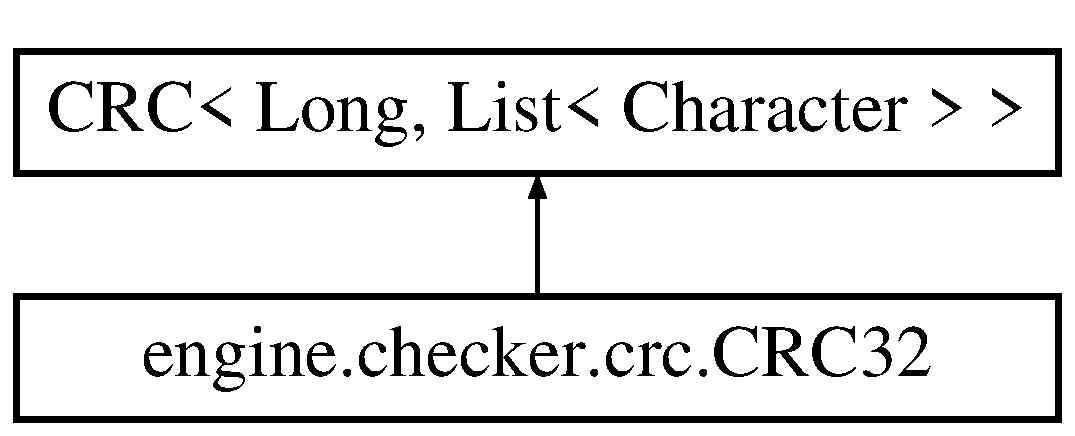
\includegraphics[height=2.000000cm]{classengine_1_1checker_1_1crc_1_1_c_r_c32}
\end{center}
\end{figure}
\subsection*{Public Member Functions}
\begin{DoxyCompactItemize}
\item 
\hypertarget{classengine_1_1checker_1_1crc_1_1_c_r_c32_a37307cfe23d0952ed53cda900209e2ca}{Long {\bfseries encode} (List$<$ Character $>$ characters)}\label{classengine_1_1checker_1_1crc_1_1_c_r_c32_a37307cfe23d0952ed53cda900209e2ca}

\end{DoxyCompactItemize}


The documentation for this class was generated from the following file\-:\begin{DoxyCompactItemize}
\item 
/\-Users/michelesummo/\-Documents/\-Git\-Hub repositories/\-P\-N\-G\-\_\-decoder/src/main/java/engine/checker/crc/C\-R\-C32.\-java\end{DoxyCompactItemize}

\hypertarget{classengine_1_1checker_1_1crc_1_1_c_r_c_3_01_numeral_type_00_01_sequence_01extends_01_list_3_04_4_01_4}{\section{engine.\-checker.\-crc.\-C\-R\-C$<$ Numeral\-Type, Sequence extends List$<$?$>$ $>$ Class Reference}
\label{classengine_1_1checker_1_1crc_1_1_c_r_c_3_01_numeral_type_00_01_sequence_01extends_01_list_3_04_4_01_4}\index{engine.\-checker.\-crc.\-C\-R\-C$<$ Numeral\-Type, Sequence extends List$<$?$>$ $>$@{engine.\-checker.\-crc.\-C\-R\-C$<$ Numeral\-Type, Sequence extends List$<$?$>$ $>$}}
}
\subsection*{Public Member Functions}
\begin{DoxyCompactItemize}
\item 
abstract Numeral\-Type \hyperlink{classengine_1_1checker_1_1crc_1_1_c_r_c_3_01_numeral_type_00_01_sequence_01extends_01_list_3_04_4_01_4_a3b8d42e3a0f86195ac310739c17fe8dc}{encode} (Sequence sequence)
\item 
boolean \hyperlink{classengine_1_1checker_1_1crc_1_1_c_r_c_3_01_numeral_type_00_01_sequence_01extends_01_list_3_04_4_01_4_a6e0509990e5c017ce3cb22d907987eaf}{check} (Sequence sequence, Numeral\-Type crc)
\end{DoxyCompactItemize}


\subsection{Detailed Description}
Classe che controlla se è stato verificato una perdita dati su una sequenza di interi.


\begin{DoxyParams}{Parameters}
{\em $<$\-Numeral\-Type$>$} & Intero di k cifre \\
\hline
{\em $<$\-Sequence$>$} & Lista di una qualsiasi sequenza di cifre \\
\hline
\end{DoxyParams}


\subsection{Member Function Documentation}
\hypertarget{classengine_1_1checker_1_1crc_1_1_c_r_c_3_01_numeral_type_00_01_sequence_01extends_01_list_3_04_4_01_4_a6e0509990e5c017ce3cb22d907987eaf}{\index{engine\-::checker\-::crc\-::\-C\-R\-C$<$ Numeral\-Type, Sequence extends List$<$?$>$ $>$@{engine\-::checker\-::crc\-::\-C\-R\-C$<$ Numeral\-Type, Sequence extends List$<$?$>$ $>$}!check@{check}}
\index{check@{check}!engine::checker::crc::CRC< NumeralType, Sequence extends List<?> >@{engine\-::checker\-::crc\-::\-C\-R\-C$<$ Numeral\-Type, Sequence extends List$<$?$>$ $>$}}
\subsubsection[{check}]{\setlength{\rightskip}{0pt plus 5cm}boolean engine.\-checker.\-crc.\-C\-R\-C$<$ Numeral\-Type, Sequence extends List$<$?$>$ $>$.check (
\begin{DoxyParamCaption}
\item[{Sequence}]{sequence, }
\item[{Numeral\-Type}]{crc}
\end{DoxyParamCaption}
)}}\label{classengine_1_1checker_1_1crc_1_1_c_r_c_3_01_numeral_type_00_01_sequence_01extends_01_list_3_04_4_01_4_a6e0509990e5c017ce3cb22d907987eaf}
Verifica se la sequenza si priva di errori.

La sequenza non deve essere vuota o nulla. La signature non deve essere vuota o nulla.


\begin{DoxyParams}{Parameters}
{\em sequence} & Sequenza di interi \\
\hline
{\em crc} & Signature crc da controllare \\
\hline
\end{DoxyParams}
\begin{DoxyReturn}{Returns}
l'esito della verifica 
\end{DoxyReturn}
\hypertarget{classengine_1_1checker_1_1crc_1_1_c_r_c_3_01_numeral_type_00_01_sequence_01extends_01_list_3_04_4_01_4_a3b8d42e3a0f86195ac310739c17fe8dc}{\index{engine\-::checker\-::crc\-::\-C\-R\-C$<$ Numeral\-Type, Sequence extends List$<$?$>$ $>$@{engine\-::checker\-::crc\-::\-C\-R\-C$<$ Numeral\-Type, Sequence extends List$<$?$>$ $>$}!encode@{encode}}
\index{encode@{encode}!engine::checker::crc::CRC< NumeralType, Sequence extends List<?> >@{engine\-::checker\-::crc\-::\-C\-R\-C$<$ Numeral\-Type, Sequence extends List$<$?$>$ $>$}}
\subsubsection[{encode}]{\setlength{\rightskip}{0pt plus 5cm}abstract Numeral\-Type engine.\-checker.\-crc.\-C\-R\-C$<$ Numeral\-Type, Sequence extends List$<$?$>$ $>$.encode (
\begin{DoxyParamCaption}
\item[{Sequence}]{sequence}
\end{DoxyParamCaption}
)\hspace{0.3cm}{\ttfamily [pure virtual]}}}\label{classengine_1_1checker_1_1crc_1_1_c_r_c_3_01_numeral_type_00_01_sequence_01extends_01_list_3_04_4_01_4_a3b8d42e3a0f86195ac310739c17fe8dc}
Crea una signature C\-R\-C.

La sequenza non deve essere vuota o nulla.


\begin{DoxyParams}{Parameters}
{\em sequence} & Sequenza di interi \\
\hline
\end{DoxyParams}
\begin{DoxyReturn}{Returns}
Signature C\-R\-C 
\end{DoxyReturn}


The documentation for this class was generated from the following file\-:\begin{DoxyCompactItemize}
\item 
/\-Users/michelesummo/\-Documents/\-Git\-Hub repositories/\-P\-N\-G\-\_\-decoder/src/main/java/engine/checker/crc/C\-R\-C.\-java\end{DoxyCompactItemize}

\hypertarget{classengine_1_1checker_1_1signature_1_1_p_n_g_signature_checker}{\section{engine.\-checker.\-signature.\-P\-N\-G\-Signature\-Checker Class Reference}
\label{classengine_1_1checker_1_1signature_1_1_p_n_g_signature_checker}\index{engine.\-checker.\-signature.\-P\-N\-G\-Signature\-Checker@{engine.\-checker.\-signature.\-P\-N\-G\-Signature\-Checker}}
}
Inheritance diagram for engine.\-checker.\-signature.\-P\-N\-G\-Signature\-Checker\-:\begin{figure}[H]
\begin{center}
\leavevmode
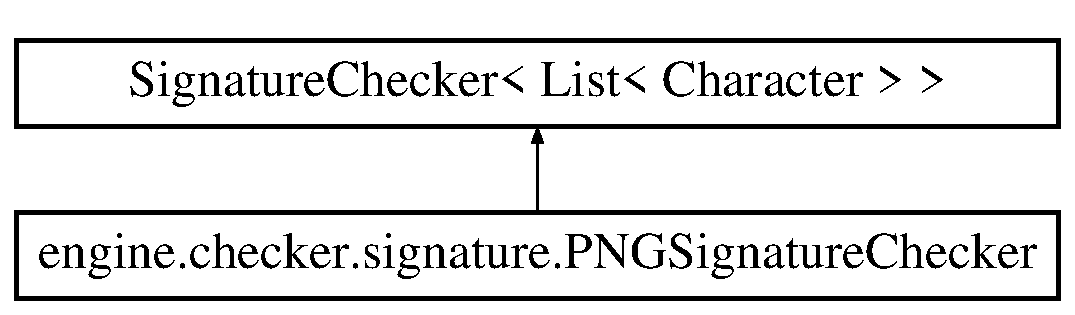
\includegraphics[height=2.000000cm]{classengine_1_1checker_1_1signature_1_1_p_n_g_signature_checker}
\end{center}
\end{figure}
\subsection*{Public Member Functions}
\begin{DoxyCompactItemize}
\item 
\hypertarget{classengine_1_1checker_1_1signature_1_1_p_n_g_signature_checker_a9d20acae12842121ca54312c5e118947}{boolean {\bfseries check} (List$<$ Character $>$ characters)}\label{classengine_1_1checker_1_1signature_1_1_p_n_g_signature_checker_a9d20acae12842121ca54312c5e118947}

\end{DoxyCompactItemize}


The documentation for this class was generated from the following file\-:\begin{DoxyCompactItemize}
\item 
/\-Users/michelesummo/\-Documents/\-Git\-Hub repositories/\-P\-N\-G\-\_\-decoder/src/main/java/engine/checker/signature/P\-N\-G\-Signature\-Checker.\-java\end{DoxyCompactItemize}

\hypertarget{interfaceengine_1_1checker_1_1signature_1_1_signature_checker_3_01_sequence_01extends_01_list_3_04_4_01_4}{\section{engine.\-checker.\-signature.\-Signature\-Checker$<$ Sequence extends List$<$?$>$ $>$ Interface Reference}
\label{interfaceengine_1_1checker_1_1signature_1_1_signature_checker_3_01_sequence_01extends_01_list_3_04_4_01_4}\index{engine.\-checker.\-signature.\-Signature\-Checker$<$ Sequence extends List$<$?$>$ $>$@{engine.\-checker.\-signature.\-Signature\-Checker$<$ Sequence extends List$<$?$>$ $>$}}
}
\subsection*{Public Member Functions}
\begin{DoxyCompactItemize}
\item 
boolean \hyperlink{interfaceengine_1_1checker_1_1signature_1_1_signature_checker_3_01_sequence_01extends_01_list_3_04_4_01_4_a8a3884735701401d87658fe87b251a25}{check} (Sequence sequence)
\end{DoxyCompactItemize}


\subsection{Detailed Description}
Classe che controlla se la firma risulta corretta.


\begin{DoxyParams}{Parameters}
{\em $<$\-Sequence$>$} & Sequenza di numeri \\
\hline
\end{DoxyParams}


\subsection{Member Function Documentation}
\hypertarget{interfaceengine_1_1checker_1_1signature_1_1_signature_checker_3_01_sequence_01extends_01_list_3_04_4_01_4_a8a3884735701401d87658fe87b251a25}{\index{engine\-::checker\-::signature\-::\-Signature\-Checker$<$ Sequence extends List$<$?$>$ $>$@{engine\-::checker\-::signature\-::\-Signature\-Checker$<$ Sequence extends List$<$?$>$ $>$}!check@{check}}
\index{check@{check}!engine::checker::signature::SignatureChecker< Sequence extends List<?> >@{engine\-::checker\-::signature\-::\-Signature\-Checker$<$ Sequence extends List$<$?$>$ $>$}}
\subsubsection[{check}]{\setlength{\rightskip}{0pt plus 5cm}boolean engine.\-checker.\-signature.\-Signature\-Checker$<$ Sequence extends List$<$?$>$ $>$.check (
\begin{DoxyParamCaption}
\item[{Sequence}]{sequence}
\end{DoxyParamCaption}
)}}\label{interfaceengine_1_1checker_1_1signature_1_1_signature_checker_3_01_sequence_01extends_01_list_3_04_4_01_4_a8a3884735701401d87658fe87b251a25}
Verifica se il file abbia una firma corretta.


\begin{DoxyParams}{Parameters}
{\em sequence} & Sequenza di numeri \\
\hline
\end{DoxyParams}
\begin{DoxyReturn}{Returns}
l'esito del controllo di tale sequenza 
\end{DoxyReturn}


The documentation for this interface was generated from the following file\-:\begin{DoxyCompactItemize}
\item 
/\-Users/michelesummo/\-Documents/\-Git\-Hub repositories/\-P\-N\-G\-\_\-decoder/src/main/java/engine/checker/signature/Signature\-Checker.\-java\end{DoxyCompactItemize}

%--- End generated contents ---

% Index
\newpage
\phantomsection
\addcontentsline{toc}{part}{Index}
\printindex

\end{document}
